\section{Measurement of inductance}
The measurement of inductance values will be done as separate part with all found resistors with
less than \(2100\Omega\).
The methode of measurement is based on the growing of current by formula \(Il~=~Imax~\cdot~(1~-~\exp{\frac{-t}{\tau}})\) 
after switching on the current.
The time constant \(\tau = \frac{L}{R}\) is proportional to the inductance~\(L\), but reverse proportional to the
resistor~\(R\). 
The current can only measured indirectly with the potential drop of a resistor.

Unfortunately the time constant will be reduced additionally by the relative high resistance \(680\Omega\),
for that the measurement of little inductance values is additionally made difficult with the \(8MHz\) clock.
To get the time constant, the voltage at the \(680\Omega\) resistor will be monitored by the analog
comparator.
If the voltage drop at the \(680\Omega\) resistor is higher than the voltage of the internal reference, this
event will be notified to the 16-bit counter, which is started at the same time of switching current on.
The counter will save the state of this event.
If the counter will overrun, this will be counted by the program.
After the event, the counter will be stopped by the program and the total time will be build with the saved
counter stage and the overflow counter.
The positive side of the coil will be switched from VCC to GND and hold in this stage until  monitoring 
of the voltages of both pins shows, that no current is detected.
The figure~\ref{fig:Inductance} shown a simplified diagram of the measurement situation.

\begin{figure}[H]
\centering

\includegraphics[]{../FIG/Inductance.eps}
\caption{Measurement of inductances with the comparator}
\label{fig:Inductance}
\end{figure}

With the supply voltage VCC and the sum of all resistors in the electric circuit the maximum current Imax and from
that the percentage of the reference voltage to the maximum voltage at the \(680\Omega\) resistor can be calculated
\(Umax~=~Imax~\cdot~(680~+~19)\) .
With the formula \(L~=~-\frac{t~\cdot~Rges}{\log{(1~-~\frac{Uref}{Umax})}}\) the inductance can be calculated.
The natural logarithm will be taken out of a build in table.
A inductance resolution of \(0.1mH\) is taken for this type of measurement.


In order to also measure lower inductance values, the \(680\Omega\) resistor will be omitted in the current loop,
if the resistance value of the inductor is measured with less than \(24\Omega\).
Only the output resistance of the port (\(19\Omega\)) will be used for measurement of the current.
In this special case the peak current will be greater than the value, that the specification of the ATmega allows.
Because this will be true only for a very short time, I expect no damage of the ATmega ports.
For this type of measurement a resolution of inductance of \(0.01mH\) is selected.
To avoid a longer time with excessive current, the additional measurement with delayed start of the counter will always be
done with the \(680\Omega\) resistor.
To get better fitting measurement results, a zero offset of 6 is subtract from the counter reading, 
if the measurement is done without the \(680\Omega\) resistor. Otherwise a zero offset of 7 or 8 is subtracted.


With great inductance values the parasitic capacity can cause a quick rise of current, so that the comparator
will responce inmmediately.
To get the value of the inductance anyway, the measurement will be repeated with a delayed start of the counter.
With this methode the voltage grow caused by the current increase of the inductor will be detected by the
analog comparator instead of the current peak of the parasitic capacity.
The measurements are always done in both current directions.
The program will select the higher result of measurement in the same current direction, but the
lower result of the different current direction as the displayed result.

\subsection{Results of the inductance measurements}
The figure~\ref{fig:Induct328p} shows the results of the measurement of different inductors.
The Inductors above \(1H\) are relays or primary sides of power transformers, for which
measurements are difficult because the iron core has residual remanence.


\begin{figure}[H]
\centering
% GNUPLOT: LaTeX picture with Postscript
\begingroup
  \makeatletter
  \providecommand\color[2][]{%
    \GenericError{(gnuplot) \space\space\space\@spaces}{%
      Package color not loaded in conjunction with
      terminal option `colourtext'%
    }{See the gnuplot documentation for explanation.%
    }{Either use 'blacktext' in gnuplot or load the package
      color.sty in LaTeX.}%
    \renewcommand\color[2][]{}%
  }%
  \providecommand\includegraphics[2][]{%
    \GenericError{(gnuplot) \space\space\space\@spaces}{%
      Package graphicx or graphics not loaded%
    }{See the gnuplot documentation for explanation.%
    }{The gnuplot epslatex terminal needs graphicx.sty or graphics.sty.}%
    \renewcommand\includegraphics[2][]{}%
  }%
  \providecommand\rotatebox[2]{#2}%
  \@ifundefined{ifGPcolor}{%
    \newif\ifGPcolor
    \GPcolortrue
  }{}%
  \@ifundefined{ifGPblacktext}{%
    \newif\ifGPblacktext
    \GPblacktexttrue
  }{}%
  % define a \g@addto@macro without @ in the name:
  \let\gplgaddtomacro\g@addto@macro
  % define empty templates for all commands taking text:
  \gdef\gplbacktext{}%
  \gdef\gplfronttext{}%
  \makeatother
  \ifGPblacktext
    % no textcolor at all
    \def\colorrgb#1{}%
    \def\colorgray#1{}%
  \else
    % gray or color?
    \ifGPcolor
      \def\colorrgb#1{\color[rgb]{#1}}%
      \def\colorgray#1{\color[gray]{#1}}%
      \expandafter\def\csname LTw\endcsname{\color{white}}%
      \expandafter\def\csname LTb\endcsname{\color{black}}%
      \expandafter\def\csname LTa\endcsname{\color{black}}%
      \expandafter\def\csname LT0\endcsname{\color[rgb]{1,0,0}}%
      \expandafter\def\csname LT1\endcsname{\color[rgb]{0,1,0}}%
      \expandafter\def\csname LT2\endcsname{\color[rgb]{0,0,1}}%
      \expandafter\def\csname LT3\endcsname{\color[rgb]{1,0,1}}%
      \expandafter\def\csname LT4\endcsname{\color[rgb]{0,1,1}}%
      \expandafter\def\csname LT5\endcsname{\color[rgb]{1,1,0}}%
      \expandafter\def\csname LT6\endcsname{\color[rgb]{0,0,0}}%
      \expandafter\def\csname LT7\endcsname{\color[rgb]{1,0.3,0}}%
      \expandafter\def\csname LT8\endcsname{\color[rgb]{0.5,0.5,0.5}}%
    \else
      % gray
      \def\colorrgb#1{\color{black}}%
      \def\colorgray#1{\color[gray]{#1}}%
      \expandafter\def\csname LTw\endcsname{\color{white}}%
      \expandafter\def\csname LTb\endcsname{\color{black}}%
      \expandafter\def\csname LTa\endcsname{\color{black}}%
      \expandafter\def\csname LT0\endcsname{\color{black}}%
      \expandafter\def\csname LT1\endcsname{\color{black}}%
      \expandafter\def\csname LT2\endcsname{\color{black}}%
      \expandafter\def\csname LT3\endcsname{\color{black}}%
      \expandafter\def\csname LT4\endcsname{\color{black}}%
      \expandafter\def\csname LT5\endcsname{\color{black}}%
      \expandafter\def\csname LT6\endcsname{\color{black}}%
      \expandafter\def\csname LT7\endcsname{\color{black}}%
      \expandafter\def\csname LT8\endcsname{\color{black}}%
    \fi
  \fi
  \setlength{\unitlength}{0.0500bp}%
  \begin{picture}(7200.00,5040.00)%
    \gplgaddtomacro\gplbacktext{%
      \csname LTb\endcsname%
      \put(814,704){\makebox(0,0)[r]{\strut{}-20}}%
      \csname LTb\endcsname%
      \put(814,1213){\makebox(0,0)[r]{\strut{}-15}}%
      \csname LTb\endcsname%
      \put(814,1722){\makebox(0,0)[r]{\strut{}-10}}%
      \csname LTb\endcsname%
      \put(814,2231){\makebox(0,0)[r]{\strut{}-5}}%
      \csname LTb\endcsname%
      \put(814,2740){\makebox(0,0)[r]{\strut{} 0}}%
      \csname LTb\endcsname%
      \put(814,3248){\makebox(0,0)[r]{\strut{} 5}}%
      \csname LTb\endcsname%
      \put(814,3757){\makebox(0,0)[r]{\strut{} 10}}%
      \csname LTb\endcsname%
      \put(814,4266){\makebox(0,0)[r]{\strut{} 15}}%
      \csname LTb\endcsname%
      \put(814,4775){\makebox(0,0)[r]{\strut{} 20}}%
      \csname LTb\endcsname%
      \put(946,484){\makebox(0,0){\strut{}10u}}%
      \csname LTb\endcsname%
      \put(1783,484){\makebox(0,0){\strut{}100u}}%
      \csname LTb\endcsname%
      \put(2619,484){\makebox(0,0){\strut{}1m}}%
      \csname LTb\endcsname%
      \put(3456,484){\makebox(0,0){\strut{}10m}}%
      \csname LTb\endcsname%
      \put(4293,484){\makebox(0,0){\strut{}100m}}%
      \csname LTb\endcsname%
      \put(5130,484){\makebox(0,0){\strut{}1 }}%
      \csname LTb\endcsname%
      \put(5966,484){\makebox(0,0){\strut{}10 }}%
      \csname LTb\endcsname%
      \put(6803,484){\makebox(0,0){\strut{}100 }}%
      \put(176,2739){\rotatebox{-270}{\makebox(0,0){\strut{}Error / Percent}}}%
      \put(3874,154){\makebox(0,0){\strut{}Inductance value / H}}%
      \put(3874,4665){\makebox(0,0){\strut{}}}%
    }%
    \gplgaddtomacro\gplfronttext{%
      \csname LTb\endcsname%
      \put(5690,4594){\makebox(0,0)[r]{\strut{}328p}}%
      \csname LTb\endcsname%
      \put(5690,4358){\makebox(0,0)[r]{\strut{}328}}%
      \csname LTb\endcsname%
      \put(5690,4122){\makebox(0,0)[r]{\strut{}168p}}%
      \csname LTb\endcsname%
      \put(5690,3886){\makebox(0,0)[r]{\strut{}168a}}%
      \csname LTb\endcsname%
      \put(5690,3650){\makebox(0,0)[r]{\strut{}168}}%
    }%
    \gplbacktext
    \put(0,0){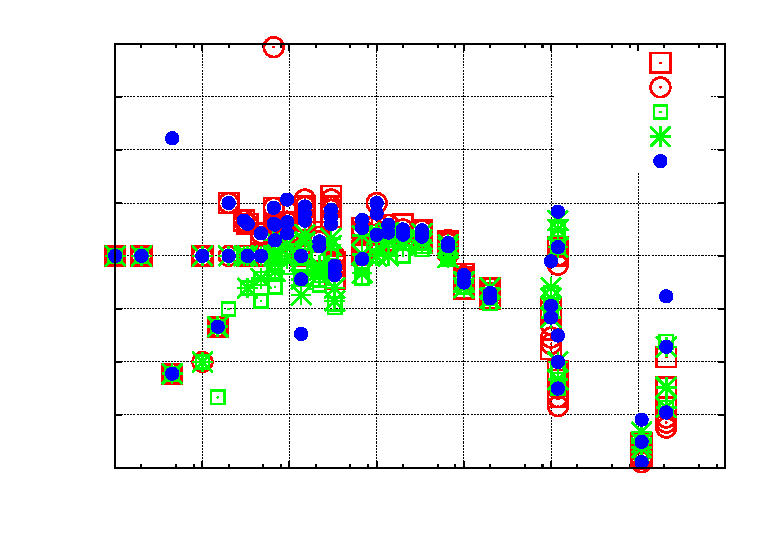
\includegraphics{../GNU/induct328p}}%
    \gplfronttext
  \end{picture}%
\endgroup

\caption{Error of inductance measurement of 15 different ATmega}
\label{fig:Induct328p}
\end{figure}

\subsection{Measurement of small inductances with the sampling method}

The smallest detectable inductance is 0.01~mH with the normal measurement technique.
For high frequency application the measurement of smaller inductances is required.
The normal method use the speed of the current grow to measure the inductance.
This method can not be used for the sampling technique, because the measurement circuit
uses no additional resistors with the coil. The current will grow to forbidden high values
very fast. We can prevent a damage of the ATmega only with a very fast break of the current flow.
For the sampling method it is difficult to get this fast current turning-off and
additionally this critical process must be done many times in series.
For this reason the radio amateur Pieter-Tjerk (PA3FWM) has used another method to
get the inductance values.
Together with a parallel connected capacitor the inductor build a resonant circuit.
With a short current pulse this circuit begins to oscillate some times without further stimulation.
With the sampling method the frequency of this oscillation can be measured.
Because one side of the coil must be connected to GND level for this measurenent,
there are two problems with the measurement.
Once the negative voltage of the oscillation is limited by the internal protection diode
of the ATmega to about 0.6~V.  
For this reason the positive part of the oscillation will never reach a higher voltage
than 0.6~V too.
Additionally the ADC of the ATmega can only measure positiv voltage values.
Therefore all negative parts of the oscillation is read as zero.
Anyway could Pieter-Tjerk find a solution, to measure the resonant frequency with
a practical precision.
With the resonant frequency the inductance can be computed, if the capacity value is known.
For this reason the calibration program is extended with a capacity measurement for
later inductance measurement use.
The capacitor will be requested with the message '' \mbox{1 \electricC 3 \(10-30nF\)(L)}''.
A default value of 18~nF is preselected for the uncalibrated tester.
The value of the parallel capacitor for inductance measurement should be selected
rather high to get a low resonant frequency with small inductance values.
A capacitor with high quality like foil-type should be selected because
the quality factor of the resonant circuit is additionally measured by
monitoring the decrease of the amplitude.
With a high quality capacitor the total quality factor of the resonant circuit
is build by the quality factor of the coil.

There is no additional operation required with the parallel connected capacitor.
The resonant circuit is usually detected automatically.
When the resonant circuit is detected, the text "if" and the expected value
of the parallel capacity is written behind the inductance value in line 2.
In this case the resistance value of the coil is written at the end of line 1.
You should check the resistance value with a separate coil measurement without
the capacitor, because the resistance measurement of the resonant circuit often fail!
A additional output line shows the measured resonant frequency and the quality factor (Q=)
of the resonant circuit.

If there is no resonant circuit detected, the resistance value and the inductance is shown
in line 2.
When a resonant frequency of a single coil is detected, the frequency value and the
quality factor of the coil is also shown in a additional line.

For a air coil with 6 turns and a parallel connected capacitor with 18~nF
the sampling method get the following result:

\begin{verbatim}
260nH if 18.1nF
2306kHz Q=38.7
\end{verbatim}

This result was measured with a operation frequency of 8~MHz. A simular result
was also measured with a 25~cm long copper wire, which was formed to one big circle.
The inductance is measured too high is this example, because the parallel capacitor
was a wound foil type with build in inductance.
The following table \ref{tab:littleInductors} shows the measurement results of some
coils with low inductance, which are all measured with a tester clocked with 16MHz.

\begin{table}[H]
\begin{center}
\begin{tabular}{| l | c | c | c | c | c |}
\hline
\hspace{1.5cm} Cp= & 6.68nF    & 11.4nF    & 18.2nF    & 20.3nF    & 33.3nF \\
Lp=           &           &           &           &           &        \\
\hline
\hline
3 turns, 13mm & 100nH     & 116nH     & 108nH     & 115nH     & 111nH  \\
 (91.4nH) & 6.039MHz  & 4.358MHz  & 3.568Mhz  & 3.282MHz  & 2.619MHz \\
              & Q=29.9    & Q=15.6    & Q=49.8    & Q=12.1    & Q=31.4  \\
\hline
4 turns, 13mm & 141nH     & 161nH     & 151nH     & 152nH     & 153nH  \\
 (144.9nH)     & 5.172MHz  & 3.724MHz  & 3.03Mhz   & 2.86MHz   & 2.226MHz \\
              & Q=44.8    & Q=16.0    & Q=46.2    & Q=14.6    & Q=30.5  \\
\hline
6 turns, 13mm & 217nH     & 232nH     & 223nH     & 224nH     & 227nH  \\
 (212.5nH)    & 4.18MHz   & 3.094MHz  & 2.492Mhz  & 2.343MHz  & 1.832MHz \\
              & Q=30.5    & Q=18.4    & Q=43.0    & Q=15.4    & Q=31.7  \\
\hline
12 turns, 13mm     & 547nH     & 571nH     & 559nH     & 560nH     & 566nH  \\
 (569.5nH)    & 2.632MHz  & 1.973MHz  & 1.573Mhz  & 1.491MHz  & 1.16MHz \\
              & Q=36.9    & Q=26.4    & Q=50.6    & Q=20.8    & Q=39.2  \\
\hline
27 turns, 11mm & \(1.93\mu H\) & \(1.92\mu H\) & \(2.02\mu H\) & \(2.00\mu H\) & \(2.01\mu H\)  \\
(\(1.9\mu H\)) & 1.403MHz  & 1.067MHz  & 828.5khz  & 789.5kHz  & 615.4kHz \\
              & Q=36.5    & Q=33.4    & Q=43.6    & Q=26.6    & Q=34.5  \\
\hline
\(6.3\mu H\)  & \(6.69\mu H\) & \(6.84\mu H\) & \(6.84\mu H\) & \(6.82\mu H\) & \(6.90\mu H\)  \\
\(7.12\mu H\) & 752.9kHz  & 570.2kHz  & 449.9khz  & 428.1kHz  & 332.3kHz \\
              & Q=28.5    & Q=30.5    & Q=32.3    & Q=25.5    & Q=28.3  \\
\hline
\end{tabular}
\end{center}
\caption{Measurement results of some coils with low inductance}
\label{tab:littleInductors}
\end{table}

The capacitors in this table are all types with low inductance like the
WIMA MKS series. With a wounded \(18.2nF\) capacitor you get a inductance of
\(196nH\) instead of the \(151nH\) from the table.
All inductors without the last one are self made coils.
The inductance value in brackets are computed values with the coil parameters.
The last \(6.3\mu H\) coils is industrial build and labled with \(6.3\mu H\).
But the measurement with a LCR-meter at 100kHz gives a result of \(7.12\mu H\)!
You can find big differences for the quality factor Q with the same coil and
different parallel capacitors with nearly the same capacity value. 
For the coil with 12 turns you see a quality factor \(50.2\) with the \(18.2nf\)
capacitor and a quality factor \(20.8\) with the \(20.3nF\) capacitor.
A program fault may be the reason for this difference.
Therefore I show the ADC data for the 12-turn coil with the \(18.2nF\) and \(20.3nF\)
capacitors in figure~\ref{fig:W12compare} for secureness.
You can find the difference of the quality factors also in the raw data clearly.
Probably the used type of the capacitor is the reason for the difference of
the quality factor.

\begin{figure}[H]
\centering
% GNUPLOT: LaTeX picture with Postscript
\begingroup
  \makeatletter
  \providecommand\color[2][]{%
    \GenericError{(gnuplot) \space\space\space\@spaces}{%
      Package color not loaded in conjunction with
      terminal option `colourtext'%
    }{See the gnuplot documentation for explanation.%
    }{Either use 'blacktext' in gnuplot or load the package
      color.sty in LaTeX.}%
    \renewcommand\color[2][]{}%
  }%
  \providecommand\includegraphics[2][]{%
    \GenericError{(gnuplot) \space\space\space\@spaces}{%
      Package graphicx or graphics not loaded%
    }{See the gnuplot documentation for explanation.%
    }{The gnuplot epslatex terminal needs graphicx.sty or graphics.sty.}%
    \renewcommand\includegraphics[2][]{}%
  }%
  \providecommand\rotatebox[2]{#2}%
  \@ifundefined{ifGPcolor}{%
    \newif\ifGPcolor
    \GPcolortrue
  }{}%
  \@ifundefined{ifGPblacktext}{%
    \newif\ifGPblacktext
    \GPblacktexttrue
  }{}%
  % define a \g@addto@macro without @ in the name:
  \let\gplgaddtomacro\g@addto@macro
  % define empty templates for all commands taking text:
  \gdef\gplbacktext{}%
  \gdef\gplfronttext{}%
  \makeatother
  \ifGPblacktext
    % no textcolor at all
    \def\colorrgb#1{}%
    \def\colorgray#1{}%
  \else
    % gray or color?
    \ifGPcolor
      \def\colorrgb#1{\color[rgb]{#1}}%
      \def\colorgray#1{\color[gray]{#1}}%
      \expandafter\def\csname LTw\endcsname{\color{white}}%
      \expandafter\def\csname LTb\endcsname{\color{black}}%
      \expandafter\def\csname LTa\endcsname{\color{black}}%
      \expandafter\def\csname LT0\endcsname{\color[rgb]{1,0,0}}%
      \expandafter\def\csname LT1\endcsname{\color[rgb]{0,1,0}}%
      \expandafter\def\csname LT2\endcsname{\color[rgb]{0,0,1}}%
      \expandafter\def\csname LT3\endcsname{\color[rgb]{1,0,1}}%
      \expandafter\def\csname LT4\endcsname{\color[rgb]{0,1,1}}%
      \expandafter\def\csname LT5\endcsname{\color[rgb]{1,1,0}}%
      \expandafter\def\csname LT6\endcsname{\color[rgb]{0,0,0}}%
      \expandafter\def\csname LT7\endcsname{\color[rgb]{1,0.3,0}}%
      \expandafter\def\csname LT8\endcsname{\color[rgb]{0.5,0.5,0.5}}%
    \else
      % gray
      \def\colorrgb#1{\color{black}}%
      \def\colorgray#1{\color[gray]{#1}}%
      \expandafter\def\csname LTw\endcsname{\color{white}}%
      \expandafter\def\csname LTb\endcsname{\color{black}}%
      \expandafter\def\csname LTa\endcsname{\color{black}}%
      \expandafter\def\csname LT0\endcsname{\color{black}}%
      \expandafter\def\csname LT1\endcsname{\color{black}}%
      \expandafter\def\csname LT2\endcsname{\color{black}}%
      \expandafter\def\csname LT3\endcsname{\color{black}}%
      \expandafter\def\csname LT4\endcsname{\color{black}}%
      \expandafter\def\csname LT5\endcsname{\color{black}}%
      \expandafter\def\csname LT6\endcsname{\color{black}}%
      \expandafter\def\csname LT7\endcsname{\color{black}}%
      \expandafter\def\csname LT8\endcsname{\color{black}}%
    \fi
  \fi
  \setlength{\unitlength}{0.0500bp}%
  \begin{picture}(7200.00,5040.00)%
    \gplgaddtomacro\gplbacktext{%
      \csname LTb\endcsname%
      \put(946,704){\makebox(0,0)[r]{\strut{} 0}}%
      \csname LTb\endcsname%
      \put(946,1383){\makebox(0,0)[r]{\strut{} 20}}%
      \csname LTb\endcsname%
      \put(946,2061){\makebox(0,0)[r]{\strut{} 40}}%
      \csname LTb\endcsname%
      \put(946,2740){\makebox(0,0)[r]{\strut{} 60}}%
      \csname LTb\endcsname%
      \put(946,3418){\makebox(0,0)[r]{\strut{} 80}}%
      \csname LTb\endcsname%
      \put(946,4097){\makebox(0,0)[r]{\strut{} 100}}%
      \csname LTb\endcsname%
      \put(946,4775){\makebox(0,0)[r]{\strut{} 120}}%
      \csname LTb\endcsname%
      \put(1078,484){\makebox(0,0){\strut{} 0}}%
      \csname LTb\endcsname%
      \put(2223,484){\makebox(0,0){\strut{} 50}}%
      \csname LTb\endcsname%
      \put(3368,484){\makebox(0,0){\strut{} 100}}%
      \csname LTb\endcsname%
      \put(4513,484){\makebox(0,0){\strut{} 150}}%
      \csname LTb\endcsname%
      \put(5658,484){\makebox(0,0){\strut{} 200}}%
      \csname LTb\endcsname%
      \put(6803,484){\makebox(0,0){\strut{} 250}}%
      \put(176,2739){\rotatebox{-270}{\makebox(0,0){\strut{}ADC value}}}%
      \put(3940,154){\makebox(0,0){\strut{}ADC sample}}%
    }%
    \gplgaddtomacro\gplfronttext{%
      \csname LTb\endcsname%
      \put(5816,4602){\makebox(0,0)[r]{\strut{}18.2nF}}%
      \csname LTb\endcsname%
      \put(5816,4382){\makebox(0,0)[r]{\strut{}20.3nF}}%
    }%
    \gplbacktext
    \put(0,0){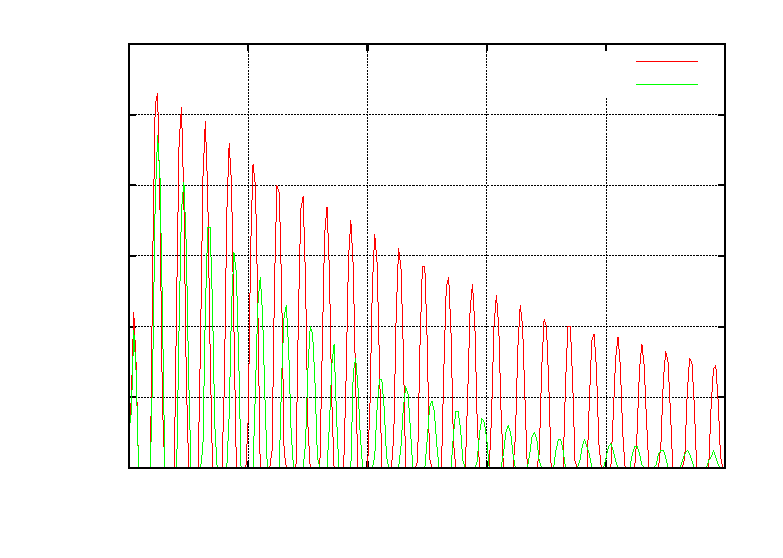
\includegraphics{../GNU/W12compare}}%
    \gplfronttext
  \end{picture}%
\endgroup

\caption{ADC data of 2 resonant circuits with the same 12 turn coil}
\label{fig:W12compare}
\end{figure}

